\documentclass[titlepage]{article}


\usepackage[T1]{fontenc}
% The preceding line is only needed to identify funding in the first footnote. If that is unneeded, please comment it out.
\usepackage{cite}
\usepackage{amsmath,amssymb,amsfonts}
\usepackage{algorithmic}
\usepackage{blindtext}
\usepackage{booktabs}
\usepackage{graphicx}
\usepackage{indentfirst}
\usepackage{textcomp}
\usepackage{titlesec}
\usepackage{xcolor}
\graphicspath{ {./images/} }
\usepackage{geometry}
\geometry{
	a4paper,
	total={170mm,257mm},
	left=20mm,
	top=20mm,
}

\def\BibTeX{{\rm B\kern-.05em{\sc i\kern-.025em b}\kern-.08em
T\kern-.1667em\lower.7ex\hbox{E}\kern-.125emX}}
\begin{document}

\title{A Lane Detection and Following System for Autonomous Vehicles\\
{\footnotesize Carleton University Engineering Capstone Group \#74}
}

\author{
	\begin{tabular}{cc}
		\begin{tabular}[t]{c}
			Curtis Davies      \\
			\texttt{101146353} \\
			\texttt{curtisrdavies@sce.carleton.ca}
		\end{tabular} &
		\begin{tabular}[t]{c}
			Liam Gaudet        \\
			\texttt{101155009} \\
			\texttt{liam.gaudet@carleton.ca}
		\end{tabular}       \\ \addlinespace[4ex]
		\begin{tabular}[t]{c}
			Ian Holmes         \\
			\texttt{101149794} \\
			\texttt{iana.holmes@carleton.ca}
		\end{tabular}       &
		\begin{tabular}[t]{c}
			Robert Simionescu  \\
			\texttt{101143542} \\
			\texttt{robert.simionescu@carleton.ca}
		\end{tabular}
	\end{tabular}
}



\maketitle
\tableofcontents


\newpage

\begin{abstract}
	\noindent Autonomous driving technology has garnered significant attention lately due to its potential to
	improve road safety and help remove the need for menial adjustments from drivers on the road.
	This project focuses on the development of a lane detection and following system for self-driving
	cars, aimed at improving a vehicle's ability to maintain its position within a lane as it drives
	along a stretch of road. \\

	\noindent The system uses a refinement-based neural network to detect and interpolate the positions of lane
	markings on the road from a real-time video feed captured by an onboard dashcam in the vehicle.
	This positional data is fed into a feedback control mechanism to generate a path for the vehicle to
	follow.
	By continuously adjusting steering commands based on the detected lane position, the system ensures
	that the vehicle remains centered within the lane. \\

	\noindent Key features of the lane detection and following system include real-time processing capabilities,
	robustness to environmental variations and driving conditions, and adaptability to different shapes
	of curves in the road. \\

	\noindent The effectiveness of the proposed system is evaluated through simulation experiments.
	Since the system is designed with modularity in mind, it can be deployed on either real hardware
	or a virtual vehicle in a simulator, allowing for detailed measuring of lane detection accuracy,
	lane-keeping precision and computational efficiency.
\end{abstract}



\section{Introduction}

The primary objective of this project is to create a system for autonomous vehicles that uses computer vision and hardware interfacing to allow the vehicle to monitor the position of lanes on its road and maintain a steady position within its own lane as it drives. 

\subsection{Identification of the Need}
Our project addresses a critical concern in autonomous vehicle development: the reliable detection and following of lanes in dynamic and diverse real-world environments. By enhancing the capabilities of autonomous vehicles to maintain their positions within lanes, our system aims to bolster road safety and reduce the need for human interaction for maintaining a steady course on trips in various kinds of roads and environmental conditions.


\subsection{Definition of the Problem}
The system is expected to function similarly to lane-following technologies in existing cars, such that they can autonomously maintain the vehicle’s position within its lane on the road on which it drives. The system is required to make the required calculations in real time and adjustments need to be smooth enough as to not introduce an unsafe level of jerk to the steering of the vehicle. 


\subsubsection{Functional Requirements}
\begin{itemize}
	\item  FR1: Lane Detection Accuracy. The system should accurately detect all lane borders within 10 centimetres of their actual position on the road 75\% of the time lane positions are calculated in a given video frame. 

TODO: Need to confirm why this number is acceptable

	\item FR2: Lane Following Precision. The system should maintain a deviation of no more than 0.45 meters from the center of its lane under normal driving conditions.

In the City of Toronto, the lane width guidelines require that the minimum lane width of any through lane be a minimum of 3.0 meters. An average sized car, which we have defined as a Honda Civic 2022, is approximately 2.1 meters wide(including mirrors). This leaves a maximum of 0.45 meters of leeway that the vehicle can deviate from the center of the lane without accidentally entering another lane.

Sources:

\begin{verbatim}
https://www.toronto.ca/wp-content/uploads/2017/11/921b-ecs-specs-roaddg-Lane_Widths_Guideline_Version_2.0_Jun2017.pdf
https://www.honda.ca/en/civic_sedan/specs
\end{verbatim}


	\item FR3: Real-time Processing
The system should complete the entire processing pipeline from video frame to hardware instruction in 150 milliseconds or less.

TODO: Provide a reasoning for why 150 milliseconds is acceptable.

\end{itemize}

\subsubsection{Non-Functional Requirements}
\begin{itemize}
	\item NFR1: Reliability. 
The system should have a minimum uptime of 99.5\% to ensure consistent operation during driving.

Since autonomous driving systems must keep the drivers safe at all times, it is imperative that the system is as reliable as possible to prevent any accidents or collisions from happening.

	\item NFR2: Compliance. 
The system should comply with any regulations and standards put in place by the Government of Ontario and the SAE for behaviour of automated driver assistance systems within vehicles.

Legal restrictions may change significantly between provinces and countries, so the legal focus of our project will be with respect to Ontario, the system the group members are most familiar with.

	\item NFR3: Extensibility. The system should provide an API that allows for programmatic control and access to its subsystems to allow any future autonomous vehicle systems to interact with it in tandem.

	\item NFR4: Documentation. 
The system should provide adequate documentation of its processes, software and runtime behaviour such that any technically-oriented person not previously affiliated with the system’s development can easily understand its functionality and inner workings.

Since this project will be build on in future years, it is imperative that the system is accessible as possible to whoever continues it. The way we intend to make that happen is by clearly documenting all of our choices within the codebase, and properly documenting any errors encountered within this report.

\end{itemize}

\subsubsection{Constraints}

The first major constraint of this project is the timeline. The duration of the project was 8 months(two four month terms), but with the final deadline being April 10th 2024 and the start date being within the first week of Fall 2023, the actual duration of the project more closely resembles 7 months. This sets a significant time constraint and was heavily accounted for when determining the work to be completed. This meant that the proper prioritization and planning of hardware acquisition, development, testing, debugging, and documentation of the system was essential due to the limited time frame. 

The team consists of four Software Engineering undergraduate students, each with varying levels and ranges of experience in software development and mostly minimal experience with electronics and hardware development. This limits what we can accomplish with respect to the hardware complexity of our system, meaning our team should focus more on the software aspect of development and use off-the-shelf hardware components.

The final major consideration for our project is the budget. Since our project has only been allocated a budget of C\$500, cost-effective solutions must be prioritized for the project. The team aims to use hardware borrowed from the school wherever possible to minimize the cost of building the system, and make use of open source systems to limit any costs associated with running the software.

\subsection{Conceptual Solutions}

\subsubsection{Literary Review}

In the landscape of commercial lane detection and following systems, several existing products and technologies exist in the public domain. Many consumer car manufacturers provide lane assistance as part of a general driver assistance system, such as Subaru’s EyeSight [1] and Honda’s Sensing [2] packages. These systems rely on camera-based vision sensors and quick image processing algorithms to detect lane markings and assist drivers in maintaining their lane position. While their the responsiveness they provide is fast and the systems work in ideal conditions, changes in light levels or unfavourable weather conditions will often render these systems completely unusable as the computer vision algorithms powering their lane detection are not sophisticated enough to detect lines without a stark contrast in light levels between the lines and the road.


On the research front, novel approaches to lane detection have gained prominence over the past 5 years, given the recent increase in capabilities of machine learning for computer vision available to small teams of developers. Approaches such as Row-wise Classification [3] of pixel data or parametric curve modeling [4] enable researchers and individuals to create model lane detection systems on hardware strong enough to run moderately complicated CNNs and other deep learning techniques. While these deep learning approaches are often more robust in varying environmental conditions, the hardware they require to process image data to extract lane position information may be too expensive for an individual researcher or for mass production in consumer-grade vehicles.

Our system needs to be robust enough to accurately and rapidly extract lane positioning information based on a video feed from the car, while avoiding the need to implant a large amount of processing hardware in the vehicle itself. Once a working model of the system is successfully implemented, the challenge will be optimizing the system to minimize its hardware footprint and the coupling between the software system and the hardware on which it is installed.

\subsubsection{Concepts}
Onboard Processing: This concept for the system would involve having a single piece of hardware perform all aspects of data processing, between lane position extraction, decision making and vehicle control interfacing. The hardware would need to be a small-enough SBC to reasonably fit in a vehicle, while also being powerful enough to handle somewhat complicated machine learning techniques. Something like the NVIDIA Jetson [5] platform may prove suitable for this task, but could be expensive given the project’s budget.

Distributed Processing: This concept involves offloading computationally expensive processes, such as deep learning image analysis, to a separate computer that is not included within the system installed in the vehicle. This allows us to use larger, more powerful hardware and have a smaller install base on our physical system. However, this would present the challenge of being able to efficiently transfer data between subsystems while minimizing latency, as this is a real-time system with a need for immediate calculations while travelling at high speeds on a road.


\subsection{System Architecture}
The overall architecture of our system is best described as a combination between a pipeline architecture and a microservice architecture. 

The pipeline nature of the system comes from the primary command flow. The system starts off by receiving an image from the camera mounted on the vehicle. The image will be processed into the software, and given to the computer vision node where the image will be analysed to determine the location of the lane lines. The location of the lanes with respect to the vehicle will be passed to the lane keeping section, where it will calculate the center of the lane and calculate the movement commands required to follow it. Then it will send the movement commands to the vehicle which will execute the instructions. 

The presence of the microservice architecture comes from the desire to clearly separate each subsystem into its own isolated component. By isolating each part of the project, individual parts become easier to develop because developers can have clearly defined contracts of inputs into the system and what they should output. Furthermore, testing the system becomes easier since each node can be tested in isolation.

\subsubsection{Software Architecture}
From a software perspective, the system can be grouped into two categories: primary subsystems, which represent major workflows in the system, and secondary subsystems, which exist only to assist the primary subsystems with their workflows but are separate components.

The two primary subsystems in our project are the Detection and the Keeping \& Control subsystems. The Detection subsystem receives raw image data from the camera and determines the vehicle location within a lane, and sends this data to the Keeping \& Control subsystem. The K\&C subsystem interprets the lane data and produces movement commands to adjust the course of the vehicle. The two subsystems are discussed further in section 3 of this proposal.

The two secondary subsystems in our project are the camera controller and the lane transformer. The camera controller is responsible for capturing the image feed from the camera mounted on the vehicle, and then supplying that to the detection node. The purpose behind this is to separate the detection module from the actual camera to remove any dependency issues. Additionally, we have a lane transformer subsystem which takes the data detected by the lane detection system and transforms it into a birds-eye view image of the lane data. The purpose of this is to simplify the operations of the primary subsystems and make it such that the primary subsystems can each be tested better in isolation.

\subsubsection{Physical Architecture}

The physical architecture for the system is a distributed system with four  significant hardware components: the camera, the onboard processing unit with ROS configured, the external processing unit with ROS configured, and the hardware/simulation for controlling the vehicle wheels. First, the camera sensor(s) capture the image data and sends that data to the onboard ROS environment. The onboard ROS environment then sends the data to an external laptop with stronger computing power which contains the software architecture described in section 1.4.1 and completes all calculations. The movement command is then sent back to the onboard processing unit which is then forwarded to the simulation or robot to execute the commands. 

\subsection{Overview of Remainder of Report}

The remainder of the report will begin with Chapter 2, which will tie the project back to the Carleton Engineering project. It starts by outlining the health and safety present as part of the project.  Then, it will detail how the team exhibited the profesionalism that is expected of engineering practitioners. The tools and systems used project management skills will also be discussed. Afterwards will be the quick discussion of how this project relates to each of the participants engineering disciplines. The section will conclude with an overview of the individual contributions made by each member of the team in both the report and the project as a whole. 

Following the Engineering Project chapter will be chapter 3, which will focus on the work plan for the project. It will include the updated work breakdown structure, followed by a responsibility matrix, an activity network, and a Gantt chart. Then, a table will detail all of the costs and any special components that were required for the project. Lastly, the risk analysis table developed at the start of the project will be reviewed.

Following the work plan will be a highlight of the two primary subsystems for the project, the Detection subsystem and the Keeping \& Control subsystem. Each subsystem will have its requirements defined. Then, the technologies and methods important to the subsystem will be discussed. Following that, the considered solutions to the subsystem will be compared and the chosen path for that subsystem will be explained. The software architecture for that subsystem will be explained, followed by an explanation as to how the subsystem was implemented and subsequently evaluated.

After the explanation of the subsystems will be a section which will discuss how all the individual subsystems were designed to fit together, and then how the system as a whole was evaluated.

Lastly, the report will conclude with a reflection done by the group which will highlight the success of the project, the significant changes from the proposal, and the groups reflections on what went wrong and what we would have done differently.

\section{The Engineering Project}

\subsection{Health and Safety}
Using the Health and Safety Guide posted on the course webpage, students will use this section to explain how they addressed the issues of safety and health in the system that they built for their project.

TODO: Review what is expected of this since health and safety is not a major consideration for the stuff we're working on

\subsection{Engineering Profesionalism}
TODO: Using their course experience of ECOR 4995 Professional Practice, students should demonstrate how their professional responsibilities were met by the goals of their project and/or during the performance of their project.

The team used their experience from ECOR 4995 to a satisfactory extent during the performance of the project. The foremost principles from this course which we made sure to follow were effectively working as a team, and ensuring sustainability in our system. 

For starters, the team did a great job at effectively working as a team. At the start of the project, the team got together and worked to best define what our objectives were for the project. After we understood the project decently well, we made sure that each member of the team had a clearly defined purpose. We also made sure to have clear and open communication with each other in case there were any issues that arose, allowing us to progress with little friction from each other.

Additionally, our team did a great job at making sure that our work was sustainable for future projects. We understood at the start of the term that our project may be used by future engineering projects, so a major part of our work was focused on making our project as accessible as possible to other individuals. This made our project more sustainable since it wouldn't compromise the ability of future projects to build on our work.

\subsection{Project Management}
One of the goals of the engineering project is real experience in working on a long-term team project. Students should explain what project management techniques or processes were used to coordinate, manage and perform their project.

The way that we approached the development of our system was focused on an agile development cycle. The purpose of this is because while we were confident with our ability to work on the project, we understood that there was a lot of risk involved in what we were trying to do. Because of that, we couldn't set fixed goals and plan too far ahead and were forced to be flexible with deadlines and accomplishing goals. In order to properly keep track of all the required tasks and objectives, we used the project management service "Click Up", see Chapter 3 for more information, which allowed us to easily track what had to be done, what dependencies existed in tasks, and track the progress on our timeline.

\subsection{Justification of Suitability for Degree Program}
In this section, students should explain how the project
relates to the degree program of each group member.

This project relates significantly to the degree of the students involved as each student is taking Software Engineering. The development of this system is entirely software based, and focuses on using many important software engineering concepts such as but not limited to project management, real-time systems, embedded systems, and machine learning. 


\subsection{Individual Contributions}
This section should carefully itemize the individual contributions of each team member. Project contributions should identify which components of work were done by each  individual. Report contributions should list the author of  each major section of this report.

\subsubsection{Project Contributions}

Curtis: 
\begin{itemize}
	\item CLRNet setup and configuration
	\item Docker setup and configuration
	\item CARLA setup and configuration
\end{itemize}

Robert: 
\begin{itemize}
	\item ROS2 configuration
	\item Configuring JetAcker
\end{itemize}

Ian:
\begin{itemize}
	\item Communication between subsystems
	\item Handling CLRNet outputs
\end{itemize}

Liam: 
\begin{itemize}
\item Controller setup and evaluation
\end{itemize}


\subsubsection{Report Contributions}
Curtis: 
\begin{itemize}
	\item Abstract
	\item Chapter 1
	\item Chapter 4.1
	\item Chapter 6
	\item LaTeX Template
\end{itemize}

Robert: 
\begin{itemize}
	\item Chapter 1
	\item Chapter 5
	\item Chapter 6
\end{itemize}

Ian:
\begin{itemize}
	\item Chapter 1
	\item Chapter 2
	\item Chapter 6
\end{itemize}

Liam: 
\begin{itemize}
\item Chapter 1
\item Chapter 4.2
\item Chapter 6
\end{itemize}

\section{Work Plan}
\subsection{Work Breakdown Structure}
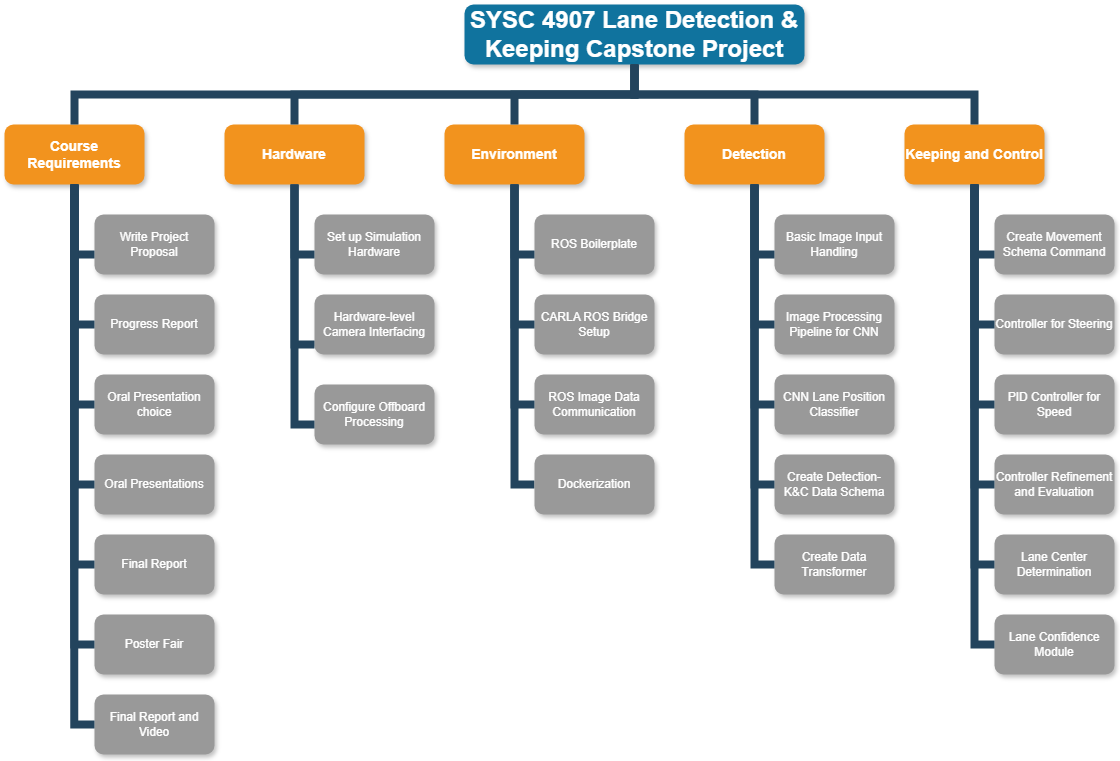
\includegraphics[width=10in,scale=1, angle=90, origin=c]{wbs.png}
\subsection{Responsibility Matrix}
\begin{center}
	\begin{tabular}{|c | c | c | c | c | c |} 
	 \hline
	 Step & Project Task & Curtis & Liam & Ian & Robert \\ [0.5ex] 
	 \hline
	 1 & Project Proposal & R & R & R & R \\ 
	 \hline
	 2 & Progress Report & R & R & R & R \\ 
	 \hline
	 3 & Oral Presentation & R & R & R & R \\ 
	 \hline
	 4 & Final Report Draft & R & R & R & R \\
	 \hline
	 5 & Poster Fair & R & R & R & R \\ 
	 \hline
	 6 & Final Report and Video & R & R & R & R \\ 
	 \hline
	 7 & Set up Simulation Software & R &  &  &  \\ 
	 \hline
	 8 & Acquire Camera Lenses & S &  & R  &  \\ 
	 \hline
	 9 & Hardware-level Camera Interfacing &  &  & R & S \\ 
	 \hline
	 10 & ROS Boilerplate &  &  &  & S \\ 
	 \hline
	 11 & CARLA ROS Bridge Setup & S &  &  & R \\ 
	 \hline
	 12 & ROS Image Data Communication & S &  &  & R \\ 
	 \hline
	 13 & Movement &  &  &  & R \\ 
	 \hline
	 14 & Basic Image Input Handling & R &  &  &  \\ 
	 \hline
	 15 & Image Processing Pipeline for CNN & R &  & S &  \\ 
	 \hline
	 16 & CNN Lane Position Classifier & R &  & S &  \\ 
	 \hline
	 17 & Lane Center Determination & R &  & S &  \\ 
	 \hline
	 18 & Create Detection-K\&C Data Schema & S &  & R &  \\ 
	 \hline
	 19 & Create Movement Schema Command &  & R &  & S \\ 
	 \hline
	 20 & PID Controller for Steering &  & R &  & S \\ 
	 \hline
	 21 & PID Controller for Speed &  & R &  & S \\ 
	 \hline
	 22 & PID Controller Refinement  &  & R &  & S \\ 
	 \hline
	 23 & MPC Controller &  & R &  & S \\ 
	 \hline
	\end{tabular}
	\end{center}
	
\subsection{Project Network}
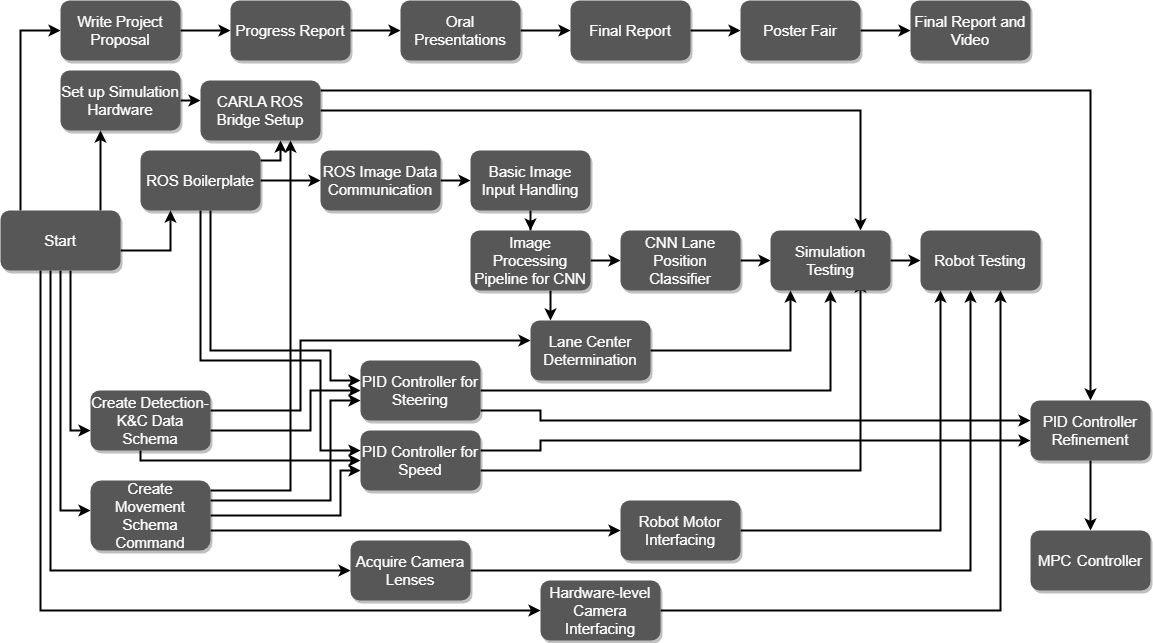
\includegraphics[width=10in,scale=1, angle=90, origin=c]{activity.png}
\subsection{Gantt Chart}
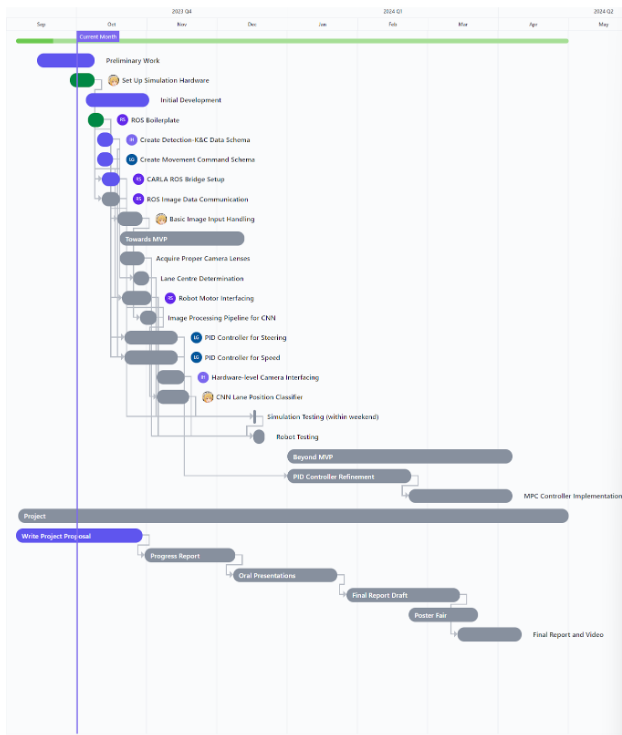
\includegraphics{gantt.PNG}
\subsection{Costs, Special Components and Facilities}
\begin{center}
	\begin{tabular}{|p{1in} | p{4in} | p{1in} |} 
	 \hline
	 Item & Description & Predicted Cost \\ [0.5ex] 
	 \hline
	 HiWOnder JetAcker & A robot that can have cameras configured onto the frame and respond to movement commands & 0\$, provided by department \\
	 \hline
	 Ubuntu Box & A Ubuntu computer capable of running the Carla Simulation software that can be accessed remotely for testing software & 0\$, provided by department \\
	 \hline
	 SSD Card & A SSD card for increasing the storage size of the HiWonder JetAcker & ~30\$ \\
	 \hline
	\end{tabular}
	\end{center}

\subsection{Risk Analysis}
TODO: Use the old risk matrix but add a column stating whether or not that error was actually encountered or not

\section{Software Subsystems}

\subsection{Lane Detection}
\subsubsection{Requirements}
\subsubsection{Technologies and Methods}
\subsubsection{Conceptualization}
\subsubsection{Software Architecture}
\subsubsection{Implementation}
\subsubsection{Evaluation}

\subsection{Lane Keeping \& Control}
The Lane Keeping \& Control (K\&C) subsystem is responsible for taking in lane position data with relation to the vehicle, determining the best corrective action to take to steer the vehicle towards the center of its lane and execute the appropriate instructions to the hardware/simulation.

\subsubsection{Requirements}
Requirement from system-wide requirements:

\begin{itemize}
	\item FR2: Lane Following Precision. The system should maintain a deviation of no more than 0.45 meters from the center of its lane under normal driving conditions.
\end{itemize}
Subsystem-specific requirements:
\begin{itemize}


	\item FR2.1: Steering Control Stability. The control subsystem should aim to minimize the heading error of the vehicle.
	
	An important part of self-driving cars is the stability of the steering. It is not desirable for the humans in the vehicle if the steering of the car is continuously changing direction and overcompensating, meaning that the control system must minimize the heading error associated with the steering.

	\item FR2.2: Control Frequency.
	The subsystem must produce movement command updates at a frequency of 50Hz.
	
	This frequency was agreed upon by the group and the project supervisors as sufficiently frequent to represent continuous feedback from the control system.
	
	\item FR2.3: Closed Loop Properties.
	The subsystem must produce movement commands using the most recent information available.

	This functional requirement is required because the rate at which the subsystem receives new lane data is not the same rate at which movement commands are required to be produced from FR2.2. This means that the system must use historical data as part of the movement commands generated at each system tick.
	
	\item FR2.4: Output Attributes. The output of the subsystem should be system agnostic and easily modifiable to any steering mechanism. 
	
	The system is not designed to be for any specific hardware system, and as such must be simple enough that it can be easily modified to fit another movement scheme.
\end{itemize}


\subsubsection{Technologies and Methods}
The development of the K\&C subsystem requires the use of three primary technologies and software concepts. 

For starters, the K\&C system will require the use of multi-threading. Multithreading is the process by which a system has multiple concurrent threads, a program in execution, running concurrently in parallel. There are several advantages of using multi-threading, including better performance due to being able to run tasks during I/O blocking time, greater scheduling flexibility, and it separates the concern of what a task does and when it does it. With respect to our system, Multithreading will need to be used to have our PID processing run in parallel to receiving new system environments from the lane detection subsystem. Multithreading was instructed as part of the SYSC 3303 Introduction to Real Time Systems course offered at Carleton. 

Another important methodology for this project is that of feedback control systems. These systems are control systems that incorporate comparing the measured variable with its target value and then manipulates the system to minimize this error[6]. Feedback control systems are advantageous since the controller takes into account any unforeseen changes present in the system such as friction from the environment or older data such as from long input processing times, both of which are likely to happen with our system[6]. These concepts are taught as part of the SYSC 3600 and SYSC 4505 courses offered at Carleton University. While these courses are not required as part of a Software Engineering degree, they can be taken as electives for students in Software Engineering and the project supervisors have experience with this concept that can be shared with the students. 

Cars and car-like vehicles use an arrangement of linkages called an Ackermann steering geometry in order to steer effectively[17]. It allows for the wheels on the inside and outside of a turn to trace circles of different radii, preventing slipping. In systems that use Ackermann steering or something similar, the front wheels turn while the rear wheels remain in place. In contrast, robots like the JetAuto use mecanum wheels, which allow for omnidirectional movement. While this is a useful property for robots, we intend to use the JetAuto to evaluate the system’s capabilities for car-like vehicles. As such, this subsystem should be able to send commands to vehicles with mecanum wheels that result in Ackerman-like movement. While this concept was not explicitly taught as part of a software engineering degree at carleton, the integration of hardware components with embedded systems relates to the practices discussed in SYSC 3310 Introduction to Real-Time Systems. 

\subsubsection{Conceptualization}

There are many different control loops that could be used to handle the lane keeping and control requirements for this sub-system. However, out of all these methods, there are two that have stood out for us as potential conceptual solutions.

PID Controller:
This control loop relies on adjustable parameters and takes in an error signal, which measures the deviation between the vehicle's position and the center of its driving lane. It then produces a sinusoidal curve with the goal of minimizing this error as rapidly as possible while avoiding excessive overshooting[13]. The main advantage of this method lies in its user-friendliness. Implementing a PID controller is straightforward as it requires only three variables for configuration, making it a preferable control system. However, a PID controller has its limitations. The main limitation with a PID controller is the limitation from only being able to tune using three parameters[14]. We anticipate that it may not be the most optimal control system due to its relatively simple configurability and handling of unexpected changes in the road path.


MPC Controller:
The MPC controller is a more sophisticated control system compared to the PID controller, with use in various industries and areas in academia.[16] It utilizes a model of the system, a cost function, and an optimization algorithm to determine the optimal strategy for minimizing error, which in this case is the distance between the car’s center and the center of its lane. One significant advantage of this controller is its potential for high accuracy when implemented effectively. The MPC controller takes a wider array of variables and information into account when making decisions, offering greater potential for improved performance metrics. However, it comes with the drawback of increased complexity. Unlike a PID controller, which is relatively straightforward to set up and configure, implementing an MPC controller involves considering a larger set of variables and a model of the environment surrounding the system, making it more challenging during the initial stages of development. 

Standford Mathematical Model(Stanley Controller):
The Stanley controller is a model based controller that calculates its recommended trajectory by using the vehicles distance to the center of the path and the heading error with the tangent line of the closest point.

Chosen Solution:
The original decision was to implement a PID controller because generally speaking, they are simple to design and implement. The intention was that after a quick PID controller was implemented, the more complex MPC controller would be implemented. Unfortunately, developing the PID controller resulted in some issues so further research was conducted and the team eventually settled on using the Stanley controller which proved to be very easy and straightforward to implement. 

\subsubsection{Software Architecture}
The Lane Keeping \& Control subsystem receives lane data from the Detection subsystem via a ROS topic using a publish-subscribe approach, allowing for asynchronous communication to accommodate different processing rates. The LaneDataListener component captures the lane position data and updates the LaneControl component. This component operates on a 50Hz timer, determining the optimal angle and velocity for the vehicle to stay centered in its lane. The output is formatted as an 
ackermann\_message
\/
AckermannDrive message, 
a data type provided by ROS, and then published to a separate ROS topic. This data is subsequently utilized by either a hardware module (simulated or real) capable of responding to Ackermann steering signals, or a software component that interprets the Ackermann steering commands and converts them into a compatible format.

\subsubsection{Implementation}
The build plan for this subsystem will begin with outlining the exact specification of the lane data that the system will receive and the exact format of the movement controls to export. This is because once these properties are established, every node in the system can be implemented in parallel rather than in series.

Following the decision of the ROS topic formats,  the listener for the lane data will be implemented. This will likely involve creating a listener for the published message, and storing it in a shared box that the PID controller can access, but the listener can write to in order to update it with the latest information.

After the listener has been implemented, the PID controller will be configured as a stub. The purpose of this is so that while the controller is being implemented, other systems can still listen to topics published by this node and receive correct data.

Next, the development of the PID controller will be performed. There are a lot of resources available for designing PID controllers, and the course notes on SYSC 3600 will provide a string foundation from which to build the controller. This is expected to take the most time to accomplish due to the high risk involved with learning and implementation. 

Once an MVP is complete, a system for using Ackermann steering messages with mecanum-wheeled vehicles to simulate Ackermann steering will be designed and implemented in order to allow control of the Hiwonder JetAuto by this system.

\subsubsection{Evaluation}
\textbf{Evaluating FR2}

When it comes to evaluating the subsystem, the most important requirement for the quality of the control system is the maximum lateral error, also known as the maximum deviation from the center of the lane.

In order to evaluate this functional requirement, a path was generated in CARLA. The vehicle would be spawned at the start of the path, and then the waypoint data would be fed to the control system as it progressed through the track. An evaluation module would record the path that the vehicle took, and after the vehicle reaches its final destination it would generate three figured and two number. The three figures represent a 2D model of the vehicles path overlayed with the waypoints, a line chart highlihgting the heading error over time, and a line chart highlighting the lateral error over time. Additionally, the evaluation node would calculate and output the highest lateral error and highest heading error. 

The control system was then evaluated by adjusting the constant speed and the controller's tuning constant each with three different values to find the one that has the lowest maximum lateral error. The results can be seen below.


The evaluation that yielded the lowest maximum lateral error was with a constant velocity of 4m/s and the tuning constant of 1.5. The error over time graphs and the 2D visualisation can be found below.


Unfortunatley, the results of this evaluation demonstrate that we did not fulfill this requirement as the conrtol system did not remain within 0.45m of the center of the lane in any tuning of the driving.

\textbf{Evaluating FR2.1}

The evaluation for determining whether or not FR2.1 was satisfied comes down to the maximum heading error velocity. The maximum heading error does not represent how much jerk si associated with the control system, but hte rate at which the error changes represents how stable the driving is. In order to evaluate this functional requirement, the same method as evaluating FR2 was performed, but instead of looking for lateral error the heading error over time was tracked to find the maximum heading error velocity.

The data from this evaluation can be found below. Overall, the system was not very stable.

\textbf{Evaluating FR2.2}

THe control frequency of hte system can be measured by having a listener to the output of hte control system. On average, the control system outputted a new message every 20ms, satisfying this requirement.

\textbf{Evaluating FR2.3}
This was accomplished by keepign a memory of the vehicles position and then letting the car drive on its own with a single datapoint to ensure that it si able to adjust its trajectory instead of using the same output as before. As a result, thsi requirement is satisfied.

\textbf{Evaluating FR2.4}
Our system outputs movement commands in the form of ackermann messages, which are easily modifiable to fit any system requirement. Therefore, this requirement is fulfilled.


\section{System Integration and Evaluation}

\subsection{Integration}
Recall that the system is made up of two primary subsystems: Lane Detection and Lane Keeping \& Control. The Lane Detection subsystem processes real-time video camera footage from a vehicle as it drives, identifies lane markers and calculates the centre of the vehicle’s lane. This information is relayed to the Keeping \& Control subsystem, which takes this data and determines the best corrective action to keep the vehicle centered in its lane. The K\&C subsystem is responsible for generating steering and acceleration commands based on the received lane position data, which is then sent to the vehicle hardware for execution. 


\subsubsection{ROS2 Orchestration}
ROS is a set of software libraries under Linux that allow for the easy orchestration and data transfer between processes running on a robot.[11] The system will use ROS as a framework for orchestrating processes, facilitating data exchange and enabling interaction with the system’s surrounding environment. ROS will serve as the backbone that synchronizes the Lane Detection and K\&C subsystems, with each subsystem running as a set of “nodes” that are managed by ROS and communicating via ROS message topics. This architecture facilitates efficient communication and coordination between the Lane Detection and K\&C subsystems. ROS topics allow the subsystems to communicate asynchronously, meaning the rate at which subsystems send messages are not dependent on one another, as they would be in a synchronous Pipeline architecture. For example, if the Keeping \& Control subsystem encounters an issue that delays sending a movement command, the next cycle will still be provided with the most recent lane information from the Detection subsystem. This is critical in a real-time implementation such as an autonomous driving system, since the vehicle will be moving at high speeds and will need to make decisions based on environmental data in a manner that is as real-time as possible to avoid lane drifting or collisions.

By incorporating ROS into our system, we gain significant benefits for its design and operation. ROS enables us to break down different tasks into separate nodes, promoting a modular approach to development. This means we can focus on specific tasks without them getting tangled up. It also helps us keep a clear track of how data moves through our system, making it easier to manage and maintain. Additionally, using ROS topics for communication allows us to interact with various hardware components for tasks like video input and vehicle control. This means we can adapt our system to different setups without having to make major changes to our codebase. This flexibility streamlines communication between our system and the environment, ensuring smoother operation of the lane detection and keeping process as the vehicle drives.


\subsubsection{Docker}
In addition to ROS, Docker was also used to assist with the integration of the software and hardware systems. A common problem with software is dependency issues, where running tasks would fail due to a dependency issue present with extenral packages. Docker solves this issue by making software run in isolated environments, makign it less likely for packaging issues to be encountered. THis helps with oru project because ther are a lot of dependency issues present with the simulation and the JetAcker, meaning containerized software is crutial to the applications success.


\subsection{Evaluation}
The system will be developed and evaluated for two phases of demonstration. The first phase will involve testing using a simulation environment, and the second will involve integration with a physical robot on a test roadway. 

The evaluation of the individual Detection and K\&C subsystems will be completed as described in sections 3.1.6 and 3.2.6 respectively. The overall evaluation of the system will involve a more high level look at the system’s functionality. 

\subsubsection{CARLA Simulator}
For the main course of the project, testing will be performed in a simulation environment using CARLA. CARLA is a driving environment simulation tool used for iterative, test-driven development of autonomous driving systems.[12] This testing method will give freedom of modifying the various parameters to be considered with respect to road conditions. Using the simulation will also allow for quick testing of features throughout development. When running simulations using CARLA, the distance from the center of the lane will be determined by the detection subsystem and adjustments to remain in the lane will be made by the K\&C subsystem. The results of the adjustments will be observed and recorded to verify proper functioning of the system. 

\subsubsection{HiWonder JetAcker}

The secondary testing for the project will include running the system on the Hiwonder JetAuto driving on a test track. The camera sensors will be mounted to the JetAuto and interfacing will be developed for communicating movement commands. Testing will be completed in a similar way to the simulation phase by observing and recording the system’s ability to maintain a sufficiently small distance from the center of the lane. 


\section{Reflections}

The final report needs to contain your original project proposal
(for example, as an Appendix or a separate chapter in your main
document). It is not uncommon that changes in your project goals
and objectives, methods used to achieve them, etc., may have
occurred over the course of the project. Therefore, in a final
chapter in the report, entitled “Reflections”, discuss how well
the original project objectives were met. Identify and discuss any
changes that occurred as the project progressed. Finally, as part
of this chapter, reflect, as a group, on the past two terms. Did
the project unfold as expected? Did the team work result in unexpected
challenges or benefits? With hindsight, if you had to undertake the
project again, would you make the same initial decisions about
tools/methods/timelines?

\subsection{Success of Project Objectives}

While we tried our best, we hit very few of our functional requirements for teh system.

\subsection{Changes from Proposal}

WE had a lot of changes from our proposal. 

Whiel we wanted ot make our own CNN, we were not able to make one on our own and had to instead use a pre-existing model.

While we initially planned to use a PID controller, it proved too complex and instead a mathematical model was used.

More...

\subsection{Group Reflection}

We bit off a lot more than we could chew. We're happy with the progress, but if we knew what we know now we would have been a lot more productive.

\section*{References}

Please number citations consecutively within brackets \cite{b1}. The
sentence punctuation follows the bracket \cite{b2}. Refer simply to the reference
number, as in \cite{b3}---do not use ``Ref. \cite{b3}'' or ``reference \cite{b3}'' except at
the beginning of a sentence: ``Reference \cite{b3} was the first $\ldots$''

Number footnotes separately in superscripts. Place the actual footnote at
the bottom of the column in which it was cited. Do not put footnotes in the
abstract or reference list. Use letters for table footnotes.

Unless there are six authors or more give all authors' names; do not use
``et al.''. Papers that have not been published, even if they have been
submitted for publication, should be cited as ``unpublished'' \cite{b4}. Papers
that have been accepted for publication should be cited as ``in press'' \cite{b5}.
Capitalize only the first word in a paper title, except for proper nouns and
element symbols.

For papers published in translation journals, please give the English
citation first, followed by the original foreign-language citation \cite{b6}.

\begin{thebibliography}{00}
	\bibitem{b1} G. Eason, B. Noble, and I. N. Sneddon, ``On certain integrals of Lipschitz-Hankel type involving products of Bessel functions,'' Phil. Trans. Roy. Soc. London, vol. A247, pp. 529--551, April 1955.
	\bibitem{b2} J. Clerk Maxwell, A Treatise on Electricity and Magnetism, 3rd ed., vol. 2. Oxford: Clarendon, 1892, pp.68--73.
	\bibitem{b3} I. S. Jacobs and C. P. Bean, ``Fine particles, thin films and exchange anisotropy,'' in Magnetism, vol. III, G. T. Rado and H. Suhl, Eds. New York: Academic, 1963, pp. 271--350.
	\bibitem{b4} K. Elissa, ``Title of paper if known,'' unpublished.
	\bibitem{b5} R. Nicole, ``Title of paper with only first word capitalized,'' J. Name Stand. Abbrev., in press.
	\bibitem{b6} Y. Yorozu, M. Hirano, K. Oka, and Y. Tagawa, ``Electron spectroscopy studies on magneto-optical media and plastic substrate interface,'' IEEE Transl. J. Magn. Japan, vol. 2, pp. 740--741, August 1987 [Digests 9th Annual Conf. Magnetics Japan, p. 301, 1982].
	\bibitem{b7} M. Young, The Technical Writer's Handbook. Mill Valley, CA: University Science, 1989.
\end{thebibliography}
\vspace{12pt}
\color{red}
IEEE conference templates contain guidance text for composing and formatting conference papers. Please ensure that all template text is removed from your conference paper prior to submission to the conference. Failure to remove the template text from your paper may result in your paper not being published.


\appendix
\end{document}
